\documentclass[10pt,aspectratio=169]{beamer}

\usetheme{Frankfurt}

\usepackage[utf8]{inputenc}
\usepackage{minted}

\title{Shimmer software architecture proposal}
\author{Matteo Cicuttin}
\institute{DISMA - PoliTO}

\begin{document}
\maketitle

\section{Intro}
\begin{frame}{Context}
    Goal: Build a tool to simulate multi-gas distribution networks

    \vspace{3mm}

    \begin{itemize}
        \item Open source tool for public dissemination
        \item Open \& documented data exchange format
        \item Interchangeable numerical models
    \end{itemize}

\end{frame}

\begin{frame}{System boundaries}

\begin{center}
    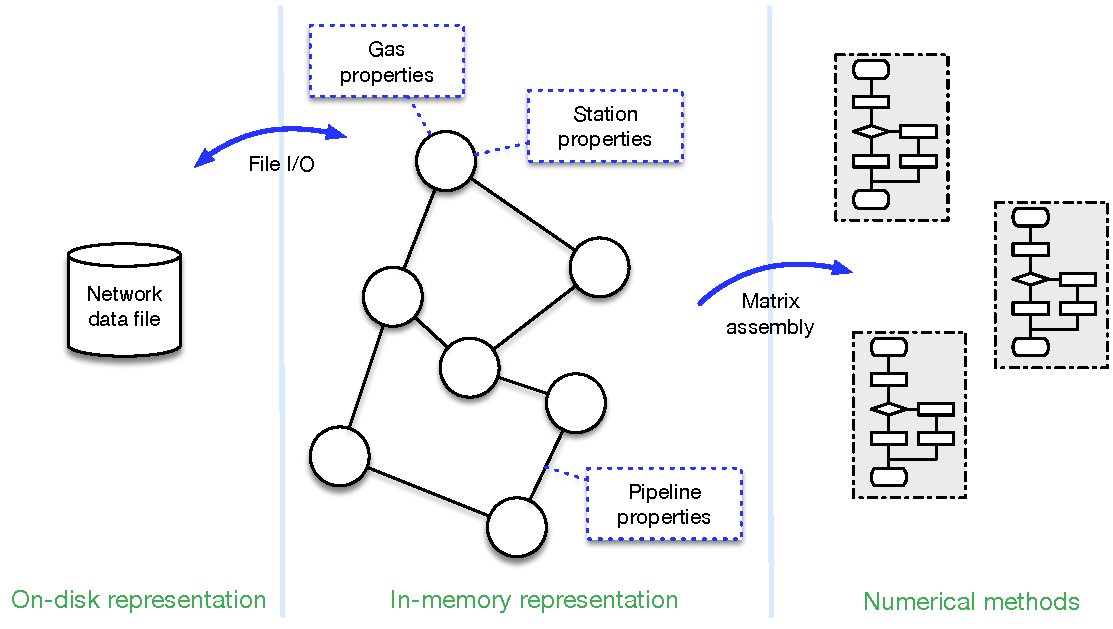
\includegraphics[width=0.8\textwidth]{img/system_arch}
\end{center}

\end{frame}

\section{Data model}

\begin{frame}{Data exchange and on-disk representation}
    Exchanging data is frequently a challenge. We want to get this right from the beginning:
    \begin{itemize}
        \item Gas network data should be stored in an \textbf{open \& well supported format}
        \item Data format should guarantee \textbf{data correctness} and \textbf{integrity}. For example:
        \begin{itemize}
            \item impossible to insert a pipe between non-existent stations
            \item impossible to remove a station with attached pipes
            \item impossible to inject a gas from a non-existent station
        \end{itemize}
    \end{itemize}

    \vspace{2mm}

    SQLite fullfills all the requirements:
    \begin{itemize}
        \item Widely supported on all main OSs and by most of the scientific tools. Example: native support in Matlab, plug-ins for Octave and R
        \item Full fledged SQL database, data constraints easily specified \& enforced
        \item Graphical tools for data manipulation \& import/export exist
    \end{itemize}
\end{frame}

\begin{frame}{Oversimplified relational data model}
    \begin{minipage}{0.6\textwidth}
        \begin{center}
            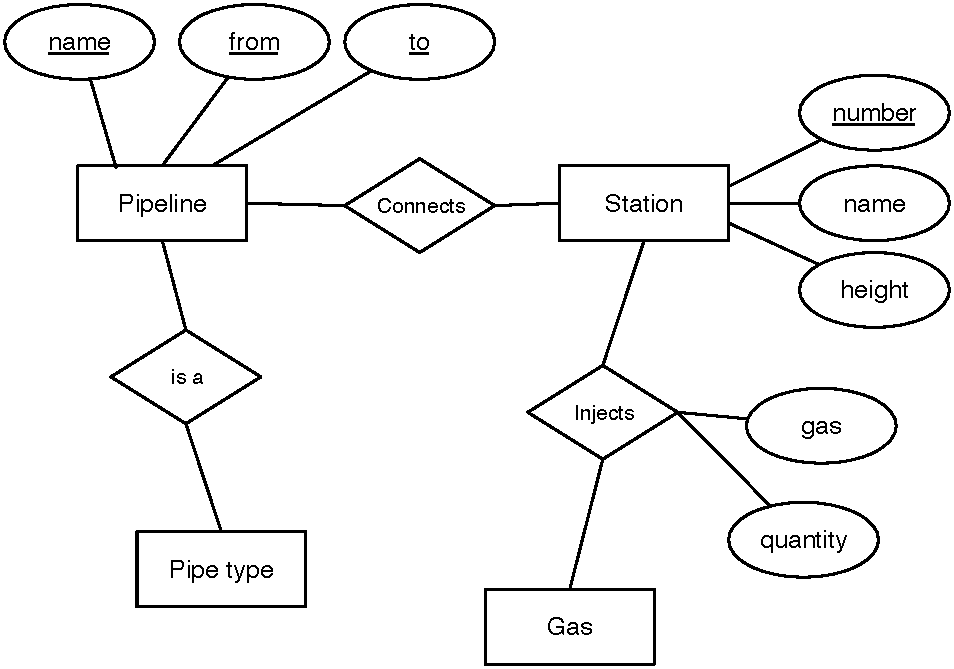
\includegraphics[width=0.9\textwidth]{img/data_arch}
        \end{center}
    \end{minipage}
    \begin{minipage}{0.39\textwidth}
        Relational data models are ubiquitous and well-understood:
        \begin{itemize}
            \item Clear and unambiguous \textbf{entities} and \textbf{relations}
            \item Data integrity automatically checked: impossible to enter an edge if a node does not exist
            \item \textcolor{red}{We need to discuss the actual data model offline in order to determine if it fits all the requirements}
        \end{itemize}
    \end{minipage}
\end{frame}

\begin{frame}[fragile]{Stations}
\begin{minted}[linenos,numbersep=5pt,frame=lines,framesep=2mm,fontsize=\footnotesize]{sql}
-- The stations. They are the nodes of the graph
create table stations (
    s_name      TEXT,
    s_number    INTEGER,
    s_height    REAL,
    PRIMARY KEY(s_number)
);
\end{minted}
\end{frame}

\begin{frame}[fragile]{Pipelines}
\begin{minted}[linenos,numbersep=5pt,frame=lines,framesep=2mm,fontsize=\footnotesize]{sql}
-- The pipelines. They are the edges of the graph.
create table pipelines (
    p_name      TEXT NOT NULL,
    s_from      INTEGER,
    s_to        INTEGER,    
    p_type      INTEGER,
    PRIMARY KEY (p_name, s_from, s_to),

    -- The source station must exist
    FOREIGN KEY (s_from)
        REFERENCES stations(s_number),
    -- The destination station must exist
    FOREIGN KEY (s_to)
        REFERENCES stations(s_number)
    -- The pipeline type must be valid
    FOREIGN KEY (p_type)
        REFERENCES pipeline_types(p_type)
);

\end{minted}
\end{frame}

\begin{frame}[fragile]{Pipeline element types}
\begin{minted}[linenos,numbersep=5pt,frame=lines,framesep=2mm,fontsize=\footnotesize]{sql}
-- Pipeline element type. Can be a pipe, a compressor, a regulator, ...
create table pipeline_types (
    p_type      INTEGER,
    t_name      TEXT NOT NULL,
    PRIMARY KEY (p_type)
);
insert into pipeline_types values (0, 'pipeline');
insert into pipeline_types values (1, 'resistor');
insert into pipeline_types values (2, 'compressor');
insert into pipeline_types values (3, 'regulator');
insert into pipeline_types values (4, 'valve');
\end{minted}
\end{frame}


\begin{frame}[fragile]{Pipeline parameters (element type 0)}
\begin{minted}[linenos,numbersep=5pt,frame=lines,framesep=2mm,fontsize=\footnotesize]{sql}
-- Pipeline parameters as length, diameter and so on.
create table pipeline_parameters (
    p_name      TEXT_NOT_NULL,
    s_from      INTEGER,
    s_to        INTEGER,
    length      REAL NOT NULL,
    diameter    REAL NOT NULL,
    epsi        REAL NOT NULL,

    -- The referenced pipeline must exist
    FOREIGN KEY (p_name, s_from, s_to)
        REFERENCES pipelines(p_name, s_from, s_to)
);
\end{minted}
\end{frame}

\begin{frame}[fragile]{Who injects what}
\begin{minted}[linenos,numbersep=5pt,frame=lines,framesep=2mm,fontsize=\footnotesize]{sql}
-- Who injects what
create table injects (
    s_number    INTEGER,
    g_name      TEXT,
    quantity    REAL,

    -- station number must be valid
    FOREIGN KEY (s_number)
        REFERENCES stations(s_number),
    -- gas name must be valid
    FOREIGN KEY (g_name)
        REFERENCES gases(g_name)
);

-- The gases. Which are the parameters associated to each gas?
create table gases (
    g_name      TEXT,
    PRIMARY KEY(g_name)
);

\end{minted}
\end{frame}

\section{In-memory representation}
\begin{frame}{In-memory representation}
    The in-memory representation is a labelled graph.
    \begin{itemize}
        \item Decouples away data handling both for input and for output
        \item Matrices for numerical methods are directly built from graph
        \item Easily implemented with \texttt{boost::graph}, graph algorithms for free
    \end{itemize}

\begin{center}
    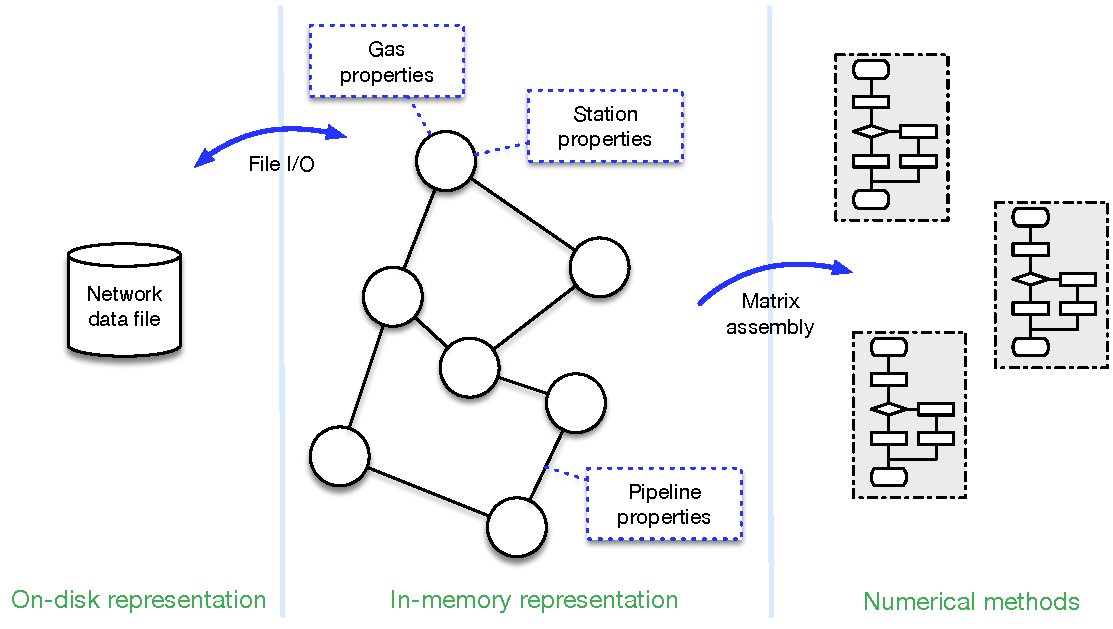
\includegraphics[width=0.5\textwidth]{img/system_arch}
\end{center}

\end{frame}
\section{Numerical models}


\section{Conclusions}

\begin{frame}{Technologies}
    We chose industry standard, portable and widespread technologies.
    \begin{itemize}
        \item SQLite for data storage and exchange: widespread format, extremely portable
        \item Data manipulation and processing
        \begin{itemize}
            \item \texttt{boost::graph} for graph manipulation
            \item Eigen for linear algebra and numerical methods
        \end{itemize}
        \item Qt to have a portable graphical toolkit and easy to install development environment
    \end{itemize}
\end{frame}

\begin{frame}{Conclusions}
    Next tasks:
    \begin{itemize}
        \item Iterate on the data model and finalize its design (DENERG/DISMA)
        \item Provide formatted \& cleaned-up data in Excel/CSV files (DENERG)
        \item Provide the first two layers of the system (DISMA)
        \item Re-implement Matlab stuff in the new architecture (DENERG/DISMA)
        \item Validate the implementation
    \end{itemize}
\end{frame}

\end{document}
